\subsection*{Redigering}
Redigering inddeles i en grænseflade og en tilhørende controller, som det fremgår af \autoref{fig:Redigering}. 

\begin{figure} [H]
\centering
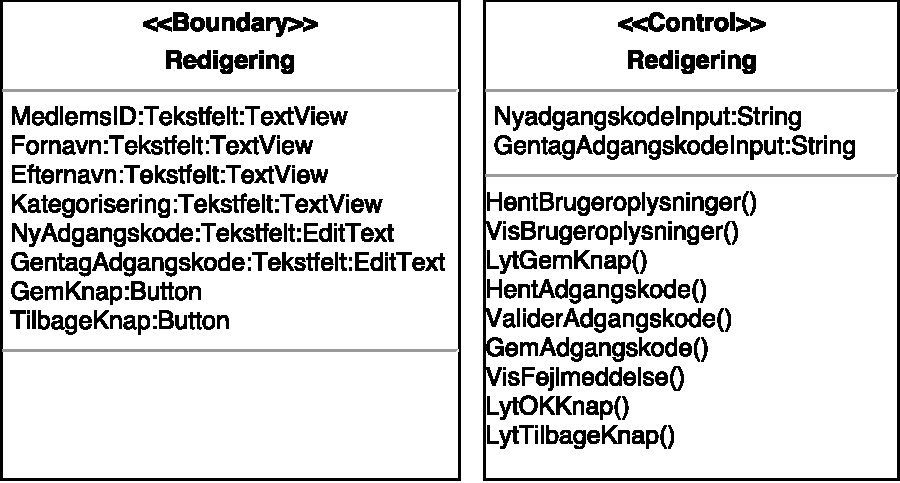
\includegraphics[width=0.9\textwidth]{figures/MVC/Redigering}
\caption{Designklasser for Redigering.}
\label{fig:Redigering}
\end{figure}

\noindent
I grænsefladen for redigering opstilles tekstfelter for medlemsID, fornavn, efternavn og kategorisering. Derudover opstilles tekstfelter for ny adgangskode og gentag adgangskode, hvor brugeren kan ændre adgangskode. Dertil er der en gem knap og en tilbage knap, af typen button. Gem knappen indikere ved tryk, at brugeren ønsker at gemme den nye adgangskode. 
Den tilhørende controller har metoder til at hente, vise, lytte, validere og gemme. Til disse klasser er der opstillet et sekvensdiagram, hvilket fremgår af \autoref{fig:SEKRedigering}.


\begin{figure} [H]
\centering
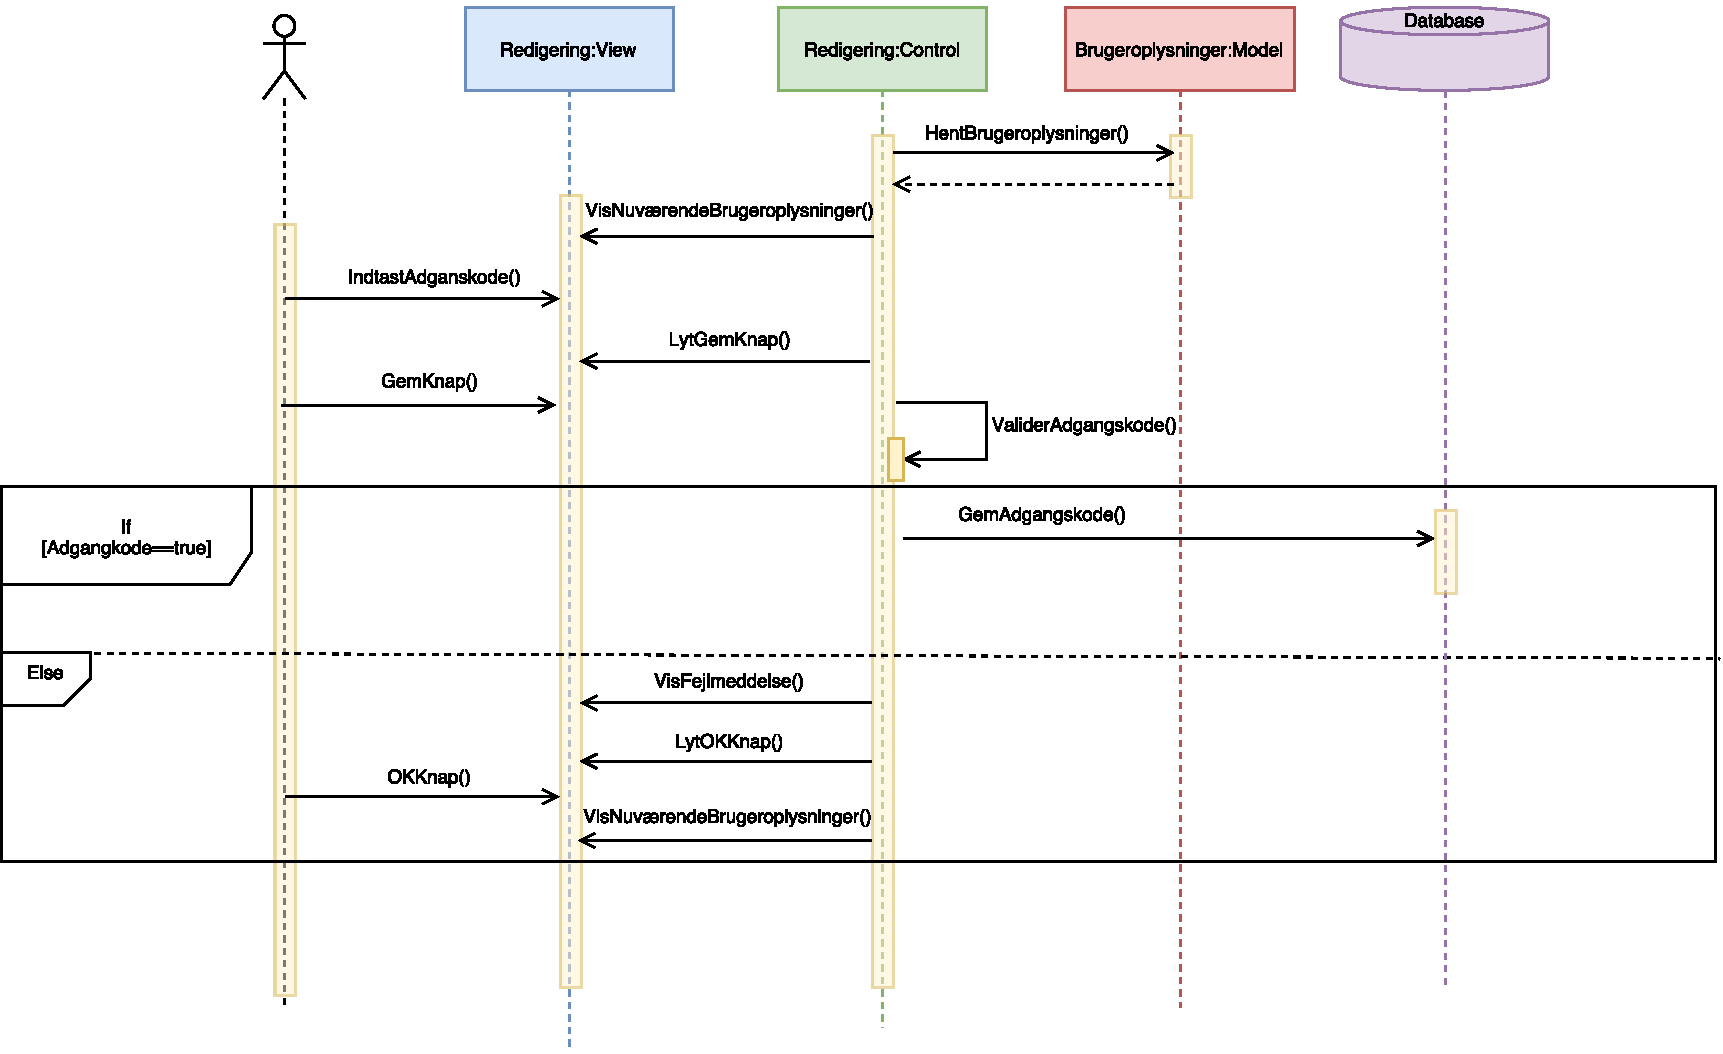
\includegraphics[width=1\textwidth]{figures/Sek/SEKRedigering}
\caption{Sekvensdiagram for redigering.}
\label{fig:SEKRedigering}
\end{figure}

\noindent
Controlleren for redigering henter brugeroplysninger fra modellen, der omfatter brugeroplysninger. Disse oplysninger vises i grænsefladen, hvortil brugeren kan se deres information. Fra denne grænseflade er det ligeledes muligt for brugeren at ændre sin adgangskoden. Adgangskoden skal indtastes to gange for at sikre, at adgangskoden er identisk. Dertil skal adgangskoden være minimum 10 karaktere lang. Adgangskoden valideres, hvis adgangskoden overholder de førnævnte kriterier, gemmes adgangskoden direkte i databasen. Adgangskoden gemmes direkte i databasen af sikkerhedsmæssig årsager, således koden ikke først gemmes idet brugeren logges ud af app'en. 
Overholder adgangskoderne derimod ikke kriterierne, vises en grænseflade for fejlmeddelelse. På denne grænseflade er der opstillet en OKKnap, der ved tryk henviser systemet tilbage til grænsefladen for redigering. 
